\documentclass[11pt,a4paper]{article}
\usepackage[utf8]{inputenc}
\usepackage[T1]{fontenc}
\usepackage[english]{babel}
\usepackage{lmodern}
\usepackage[margin=2.2cm]{geometry}
\usepackage{booktabs}
\usepackage{graphicx}
\usepackage{enumitem}
\usepackage{hyperref}
\setlist{itemsep=0.1em, topsep=0.2em}
\setlength{\parskip}{0.25em}
\setlength{\parindent}{0pt}

\title{\vspace{-1.5em}Blind Spot: Milestone M1\\[0.2em]
  \large Test set, evaluation framework and offline pipeline with base model}
\author{Mika Brückner, Yannik Köllmann\\[0.2em]
  \small Anwendungspraktikum 3D-Rechnersehen / Projekt \glqq Intelligente Systeme\grqq}
\date{24 November 2026}

\begin{document}
\maketitle
\vspace{-1.5em}

\section*{Project status}

\textbf{Data (WP 1.1--1.4).} The SANPO loader reads the real chest-camera sessions with depth in meters and
intrinsics matched to the depth resolution. Session-level train, val and test splits and obstacle annotations
for 40 SANPO test frames, derived from SANPO's panoptic masks, are in review. We recorded
14 sequences of our own with the iPhone~12~Pro and the Stray Scanner app (6 indoor, 7 on a terrace, 1 door
transition; day and night), with LiDAR depth as ground truth and ARKit intrinsics per frame. Recording names encode
environment, scene, lighting and obstacle types, so every metric can be grouped by them. The camera height on the chest is measured at 1.30\,m. Not done yet: annotations of our own
recordings, outdoor recordings on real sidewalks and streets, and separate training recordings.

\textbf{Evaluation framework (WP 5.1).} One command runs any set of models over SANPO and our recordings and
writes a JSON and Markdown report plus performance figures for slides and documents. It measures AbsRel, RMSE and $\delta_1$ per
depth range (0--2, 2--5, 5--10\,m), error over distance, parameters, latency and peak memory, and the alert
metrics (recall, false alarm rate, direction, distance error) as soon as annotations exist. The framework is covered by 62 tests that run in CI
without GPU, network or model weights.

\textbf{Model comparison (WP 2.1).} We integrated 14 pretrained models behind one interface that receives the
image and the camera intrinsics, but never the ground truth. They fall into three groups: metric models
without camera information (e.g.\ Depth Anything~V2 Metric, YOLO26n), metric models that use the focal length
(e.g.\ Metric3D~v2, UniDepthV2) and relative models (e.g.\ MiDaS, ZipDepth).
All ran on 528 frames (45 SANPO, 483 own); the small models also run on the CPU with identical results.
Without help, the small models get only $\delta_1 = 0.39$--$0.55$ on our recordings ($\delta_1$: share of
pixels within 25\,\% of the LiDAR depth). With one correct scale factor per frame, an upper bound for the
planned ground scaling, the models that use the focal length reach about 0.90 (UniDepthV2~S at 15\,ms,
Metric3D~S at 65\,ms, MoGe-2~S at 45\,ms on an RTX~5070~Ti), DA~V2 Metric Indoor~S 0.85, YOLO26n 0.77 and
the relative DA~V2 Small and ZipDepth 0.76 and 0.74 (Figure~\ref{fig:speed}). Depth Anything~3 Metric Large
is the most accurate model (0.86 raw, 0.93 scaled), but with 334\,M parameters too large for the phone.

\begin{figure}[t]
\centering
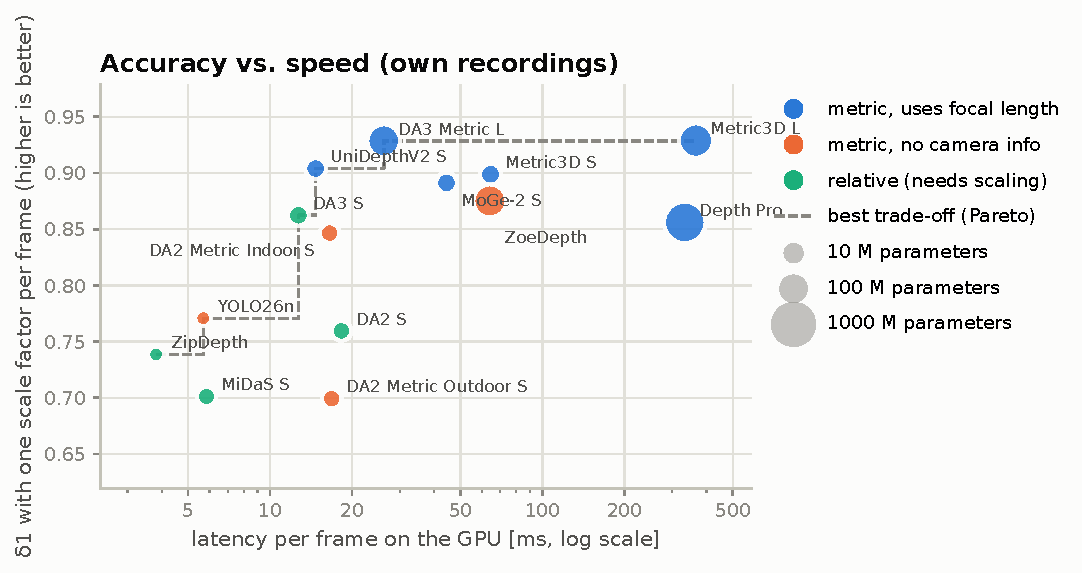
\includegraphics[width=0.92\linewidth]{figures/m1_accuracy_vs_latency.pdf}
\caption{Accuracy with one scale factor per frame over GPU latency on our recordings. Dashed: best
trade-off; point size: number of parameters.}
\label{fig:speed}
\end{figure}

We have not fixed a single base model yet. We carry the best model of each group into ground scaling (WP 2.2):
UniDepthV2~S (accuracy of Metric3D~S at a quarter of its latency), DA~V2 Metric Indoor~S and DA~V2 Small. The
final choice depends on how they behave with ground scaling and whether they can be exported to and run on the
iPhone; Depth Anything~3 Metric Large serves as a reference and as a possible teacher for fine-tuning (WP 2.3).

\textbf{Alert logic (WP 3.1, own branch).} The offline pipeline goes from image over depth to alerts. A walking corridor in
3D (0.9\,m wide, ground and points above head height removed using camera height and pitch) raises an alert
for the left, center or right third of the image when enough points lie closer than 3\,m; a naive baseline
without corridor serves as comparison. How good the alerts are can only be measured once our recordings are
annotated.

\section*{New insights}

\begin{itemize}[leftmargin=1.2em]
\item \textbf{Scale is the main problem, not structure.} Without help, the small models reach only
  $\delta_1 = 0.39$--$0.55$ on our recordings; with one correct scale factor per frame, the same predictions
  reach 0.85--0.90. Ground scaling (WP 2.2) is therefore the most important next step. Models that use the
  focal length profit most from it. Relative models also need a shift, not only a scale, so the ground fit has
  to estimate both.
\item \textbf{The near range is the weak spot.} All models are worst below 1\,m, exactly where alerts matter.
  SANPO cannot measure this: its stereo depth starts at about 2\,m, and its test frames contain almost no
  obstacles in the walking path within 3\,m. Our own LiDAR recordings are indispensable, but the LiDAR is
  only reliable up to about 5\,m (99.9\,\% of the valid pixels lie below 5.1\,m).
\item \textbf{Lighting matters more than indoor versus outdoor.} At night the scaled $\delta_1$ of Metric3D~S
  drops from 0.93 to 0.83. Routing to separate indoor and outdoor models would not help: the indoor variant of
  Depth Anything~V2 Metric beats its outdoor variant even outdoors, and ZoeDepth, which routes internally, is
  poor outdoors.
\item \textbf{Every data source needs a check against real data.} SANPO depth files carry an undocumented
  header and a lower resolution than the images. The iPhone videos decode one frame fewer than there are depth
  maps; correlating camera rotation with image motion showed that the first frame is missing, so image and
  depth would otherwise have been off by one frame.
\item \textbf{Evaluation choices change the ranking.} Scaling relative models with a single factor makes them
  look far worse than they are (Depth Anything~V2 Small: $\delta_1 = 0.76$ versus 0.94 with scale and shift), and a few far-off pixels
  (Depth Pro in front of walls) dominated the mean until predictions were clipped to the evaluated range.
  Oracle alignments must be labeled as upper bounds.
\item \textbf{Research code is fragile.} Pretrained models came with CUDA-only code, conflicting version pins
  and even an interactive prompt that silently blocked a run; separate environments, pinned commits and a
  shared prediction cache keep the comparison reproducible.
\item \textbf{In hindsight}, we would record real sidewalks earlier and test every loader on real files first.
\end{itemize}

\end{document}
